\documentclass[a4paper,12pt]{extarticle}
\usepackage[backend=bibtex]{biblatex}
\addbibresource{mybib.bib}
\usepackage{pgfplots}
\pgfplotsset{compat=1.9}
\usepackage[utf8]{inputenc}
\usepackage[T1,T2A]{fontenc}
\usepackage[english,russian]{babel}
\usetikzlibrary{babel}
\usepackage{graphicx}
\usepackage{wrapfig}
\usepackage{hyperref}
\usepackage{hhline}
\usepackage{multirow}
\usepackage{amsmath,amsfonts,amssymb,amsthm,mathtools}
\usepackage{wasysym}
\usepackage{listings}
\lstset{language=Python}
\usepackage{setspace}
\usepackage[left=1.5cm,right=1.5cm,top=2cm,bottom=2cm]{geometry}
\linespread{1.3}
\usepackage{csquotes}
\usepackage{bchart}
\usepackage{pgf-pie}
\usepackage{tikz}
\usepackage[user,titleref]{zref}
\usepackage{enumitem}
\usetikzlibrary{shadows}
\usepackage{caption}
\usepackage{minted}
\usepackage{subcaption}
\usepackage{multicol}
\usepackage{cleveref}

\begin{document}
\begin{titlepage}

  \thispagestyle{empty}

  \centerline{\large{XXIII Международная конференция научно-технических работ школьников}}
  \centerline{\large{<<Старт в Науку>>}}

  \vfill

  \begin{center}
    \Huge\textbf{ИССЛЕДОВАТЕЛЬСКАЯ РАБОТА} \\
    \Large{на тему:} \\
    \Large{Алгоритм нахождения наибольшей общей подпоследовательности для нескольких последовательностей\\Linear-MLCS}
  \end{center}

  \begin{flushright}
    \vskip 3in
    \begin{tabular}{l}
      \textbf{Выполнил:}\\Ученик Ришельевского научного лицея\\Сидюк Дмитрий Андреевич\\\\\\
      \textbf{Научный руководитель:}\\Сидюк Андрей Анатольевич\\Senior AI developer (math apparatus)\\ROMAD Cyber Systems Inc.
    \end{tabular}
    \vskip 0.5in
  \end{flushright}

  \centerline{Одесса-2021}

\end{titlepage}

\tableofcontents

\printbibliography[heading=bibintoc]

\thispagestyle{empty}

\setcounter{page}{1}

\clearpage

\section{Введение}

Информация в различных своих проявлениях часто выражается в виде последовательностей элементов с конечным алфавитом, что порождает необходимость находить их наибольшие общие подпоследовательности. Будь то цепочка ДНК здорового человека и человека с генетическими отклонениями, паттерны поведения приложений и вредоносных программ, сравнение файлов и т.д. Для решения данной задачи было создано множество алгоритмов. Однако все эти решения объединяет серьезная проблема — они невероятно ресурсозатратные, требуют много памяти и времени для работы.

С современными темпами развития технологий объемы данных стремительно растут, что требует поиска более оптимальных решений проблемы поиска наибольших общих подпоследовательностей. В данной работе будет рассмотрен Linear-MLCS алгоритм, который заключается в построение неизбыточного графа наибольших общих подпоследовательностей \textit{Non-redundant Common Subsequence Graph} (NCSG) с дальнейшими его прямой и обратной топологическими сортировками для устранения сопутствующих дефектов. Данный алгоритм намного эффективнее аналогов в использовании места и времени необходимого для работы, к тому же он позволяет найти абсолютно все возможные наибольшие общие подпоследовательности \textit{Multiple Longest Common Subsequence} (MLCS) для неограниченного количества последовательностей.

Целью данной работы является реализация алгоритма Linear-MLCS на языках программирования Python и C++, а так же исследование некоторых зависимостей в полученных с его помощью последовательностях.

\section{Реализация алгоритма на языке Python}
Для наглядной демонстрации работы алгоритма реализуем его на языке Python.
Принцип действия алгоритма состоит из 6 основных частей:
\begin{enumerate}
  \item Избавление от уникальных элементов
  \item Построение таблиц
  \item Построение NCSG
  \item Сортировка NCSG
  \item Чтение NCSG
\end{enumerate}

Рассмотрим каждую из частей на примере трех последовательностей
\[S_{1} = TFGACGADTC \quad S_{2} = ATGLCTCAFG \quad S_{3} = CTADGTALCG\]
с алфавитом используемым на практике для описания цепочек ДНК $\Sigma_{4} = \left\{A, C, G, T\right\}$

\subsection{Избавление от уникальных элементов}
\label{preproc}

Прежде всего следует избавиться от уникальных элементов последовательностей, т.к. элементы не содержащиеся во всех исходных последовательностях не могут содержаться и в их подпоследовательностях. Т.е. нужно удалить элементы отмеченные красным цветом

\[S_{1} = T\textcolor{red}{F}GACGA\textcolor{red}{D}TC \quad S_{2} = ATG\textcolor{red}{L}CTCA\textcolor{red}{F}G \quad S_{3} = CTA\textcolor{red}{D}GTA\textcolor{red}{L}CG\]

Для достижения данной цели напишем следующую функцию:

\begin{minted}[fontsize=\footnotesize, frame=lines, breaklines, breakafter=d, fontsize=\footnotesize, linenos]{python}

def Preprocessing(self, Sequences): #В функцию передается список исходных последовательностей
    if len(Sequences) > 0: #Проверяем, не пуст ли переданный список
        self.alphabet = set(Sequences[0]) #Запоминаем алфавит первой последовательности из списка
        for i in range(1, len(Sequences)): #Перебираем остальные последовательности
            self.alphabet = self.alphabet.intersection(Sequences[i]) #Удаляем уникальные элементы
    else:
        return()
    res = []
    for i in range(len(Sequences)):
        res.append([s for s in Sequences[i] if s in self.alphabet]) #Составляем обновленный список последовательностей
    return(res)

\end{minted}

\begin{minted}[fontsize=\footnotesize, frame=lines, breaklines, breakafter=d, fontsize=\footnotesize, linenos]{python}

>>> data = [list('TFGACGADTC'), list('ATGLCTCAFG'), list('CTADGTALCG')]
>>> dataPreprocessed = Preprocessing(data)
>>> dataPreprocessed
[['T', 'G', 'A', 'C', 'G', 'A', 'T', 'C'], ['A', 'T', 'G', 'C', 'T', 'C', 'A', 'G'], ['C', 'T', 'A', 'G', 'T', 'A', 'C', 'G']]

\end{minted}

Полученные последовательности без уникальных элементов

\[S_{1} = TGACGATC \quad S_{2} = ATGCTCAG \quad S_{3} = CTAGTACG\]

мы используем в дальнейшем для построения таблиц Successor Tables.

\subsection{Построение таблиц}

Следующим шагом необходимо построить таблицы Successor Tables для каждой из последовательностей, ориентируясь на которые в дальнейшем будет построен NCSG. Построим таблицы следующей функцией:

\begin{minted}[fontsize=\footnotesize, frame=lines, breaklines, breakafter=d, fontsize=\footnotesize, linenos]{python}

def SuccessorTable(self, Sequences): #На вход функции передается список последовательностей
    res = []
    for i in range(len(Sequences)): #Рассматриваем каждую последовательность по очереди
        currTable = {char: [] for char in self.alphabet} #Создаем словарь, ключами которого являются элементы алфавита
        for j in range(len(Sequences[i])): #Перебираем элементы текущей последовательности
            for key in currTable.keys(): #Перебираем алфавит
                try:
                    pos = Sequences[i][j:].index(key) + j #Получаем позицию первого вхождения элемента алфовита key после текущего элемента последовательности j

                except:
                    continue #Если таких вхождений нет, переходим к следующему элменту алфавита
                currTable[key].append(pos+1) #Формируем таблицу, заполняя её индексами первых вхождений текущего элемента алфавита после текущего элемента последовательности j
        res.append(currTable) #В переменную res записываем получившиеся таблицы, которые и возвращает функция
    return(res)

\end{minted}

В нашем случае нужно построить 3 таблицы, левые столбцы которых заполняются элементами алфавита $\Sigma_{4} = \left\{A, C, G, T\right\}$, а верхние строки нулем и далее элементами последовательностей полученных в пункте \ref{preproc} с их соответствующими индексами начиная с единицы. Далее строка с каждым элементом алфавита заполняется номерами следующих вхождений данного элемента в последовательности. Итоговые таблицы для последовательностей $S_{1}$, $S_{2}$ и $S_{3}$ представлены в \hyperref[table:1]{приложении 1}.

\begin{table}[h!]
  \centering
  \caption*{\textbf{Приложение 1: }Successor Tables для рассматриваемых последовательностей $S_{1}$, $S_{2}$ и $S_{3}$}
  \phantomsection
  \addcontentsline{toc}{subsubsection}{\textbf{Приложение 1: }Successor Tables для последовательностей $S_{1}$, $S_{2}$ и $S_{3}$}
  \label{table:1}
  \renewcommand{\arraystretch}{1.5}
  \renewcommand{\tabcolsep}{0.25cm}
  \begin{tabular}{ c | c | c | c | c | c | c | c | c | c |}
    $S_{1}$ & $=$ & T & G & A & C & G & A & T & C \\
            & 0 & 1 & 2 & 3 & 4 & 5 & 6 & 7 & 8 \\
    \hline
    A & 3 & 3 & 3 & 6 & 6 & 6 & - & - & - \\
    \hline
    C & 4 & 4 & 4 & 4 & 8 & 8 & 8 & 8 & - \\
    \hline
    G & 2 & 2 & 5 & 5 & 5 & - & - & - & - \\
    \hline
    T & 1 & 7 & 7 & 7 & 7 & 7 & 7 & - & - \\
    \hline
  \end{tabular}
\end{table}
\begin{table}[h!]
  \hspace{-1.5cm}
  \centering
  \renewcommand{\arraystretch}{1.5}
  \renewcommand{\tabcolsep}{0.25cm}
  \begin{tabular}{ c | c | c | c | c | c | c | c | c | c |}
    $S_{2}$ & $=$ & A & T & G & C & T & C & A & G \\
            & 0 & 1 & 2 & 3 & 4 & 5 & 6 & 7 & 8 \\
    \hline
    A & 1 & 7 & 7 & 7 & 7 & 7 & 7 & - & - \\
    \hline
    C & 4 & 4 & 4 & 4 & 6 & 6 & - & - & - \\
    \hline
    G & 3 & 3 & 3 & 8 & 8 & 8 & 8 & 8 & - \\
    \hline
    T & 2 & 2 & 5 & 5 & 5 & - & - & - & - \\
    \hline
  \end{tabular}\hspace{1cm}
  \begin{tabular}{ c | c | c | c | c | c | c | c | c | c |}
    $S_{3}$ & $=$ & C & T & A & G & T & A & C & G \\
            & 0 & 1 & 2 & 3 & 4 & 5 & 6 & 7 & 8 \\
    \hline
    A & 3 & 3 & 3 & 6 & 6 & 6 & - & - & - \\
    \hline
    C & 1 & 7 & 7 & 7 & 7 & 7 & 7 & - & - \\
    \hline
    G & 4 & 4 & 4 & 4 & 8 & 8 & 8 & 8 & - \\
    \hline
    T & 2 & 2 & 5 & 5 & 5 & - & - & - & - \\
    \hline
  \end{tabular}
  \hspace{-1.5cm}
\end{table}

\subsection{Построение NCSG}

Теперь, имея таблицы мы можем построить \textit{Non-redundant Common Subsequence Graph} (NCSG), дальнейшее чтение которого и позволит найти наибольшие общие подпоследовательности для нескольких последовательностей \textit{Multiple Longest Common Subsequenc} (MLCS). Для построения NCSG напишем следующую функцию:

\begin{minted}[fontsize=\footnotesize, frame=lines, breaklines, breakafter=d, fontsize=\footnotesize, linenos]{python}

def ConstructedNCSG(self, tables, data): #На вход функции передаются таблицы Successor Tables, а так же список отсортированных последовательностей
    self.sourcePoint = tuple([0 for _ in data]) #Формируем нулевую, начальную точку
    self.sinkPoint = tuple([65535 for _ in data]) #Формируем конечную точку
    level_keys = set() #Множество вершин текущего слоя
    level_keys.add(self.sourcePoint) #Первый слой состоит только из начальной точки
    self.ncsg[self.sourcePoint] = {'char': '', 'out': set(), 'in': set()} #Формируем NCSG, к каждой вершине NCSG привязано множество входящих и исходяцих вершин, а так же элемент алфавита
    while len(level_keys) > 0: #Временная переменная с вершинами текущего слоя
        tmp_keys = set() #Временная переменная с вершинами текущего слоя
        for key in level_keys: #Перебираем вершины последнего найденного слоя
            for char in self.alphabet: #Перебираем элементы алфавита
                link = [] #Временная переменная с координатами текущей вершины
                for i in range(len(tables)): #Перебираем таблицы
                    try:
                        link.append(tables[i][char][key[i]]) #Для каждой вершины, начиная с исходной (0, 0, 0), в соответствующих её координатам таблицах для каждого элемента алфавита находим координаты новых вершин с которыми данная вершина имеет связь
                    except:
                        link = self.sinkPoint #Если искомой координаты нет, значит мы пришли в конечную точку NCSG
                        break
                link = tuple(link) #Преобразуем полученные координаты вершины в кортеж
                if (link != self.sinkPoint) and (not link in self.ncsg):
                    tmp_keys.add(link)
                if not link in self.ncsg:
                    self.ncsg[link] = {'char': char, 'out': set(), 'in': set()}
                self.ncsg[link]['in'].add(key) #Добавляем связь, входящую в найденную вершину из предыдущей
                self.ncsg[key]['out'].add(link) #Добавляем связь, исходящую из предидущйе вершины в найденную
        level_keys = tmp_keys #Определяем список найденных вершин нового слоя

\end{minted}

Рассмотрим построение NCSG по-порядку. Сначала искусственно зададим начало графа — точку (0, 0, 0). Далее выберем таблицу для первой последовательности $S_{1}$ и любой элемент алфавита, например элемент <<A>>. Теперь рассмотрим координаты текущей, в данном случае первой, начальной точки. Первая координата — $0$, значит находим число в \hyperref[table:2]{первой таблице} по ключу A и индексу $0$. Это число — $3$, в \hyperref[table:2]{приложении 2} оно выделено красным цветом.
\begin{table}[h!]
  \centering
  \caption*{\textbf{Приложение 2: }Successor Table для последовательности $S_{1}$ и элемента <<A>>}
  \phantomsection
  \addcontentsline{toc}{subsubsection}{\textbf{Приложение 2: }Successor Table для последовательности $S_{1}$ и элемента <<A>>}
  \label{table:2}
  \renewcommand{\arraystretch}{1.5}
  \renewcommand{\tabcolsep}{0.25cm}
  \begin{tabular}{ c | c | c | c | c | c | c | c | c | c |}
    $S_{1}$ & $=$ & T & G & A & C & G & A & T & C \\
            & 0 & 1 & 2 & 3 & 4 & 5 & 6 & 7 & 8 \\
    \hline
    A & \textcolor{red}{3} & 3 & 3 & \textcolor{teal}{6} & 6 & 6 & - & - & - \\
    \hline
  \end{tabular}
\end{table}

\noindent Вторая координата это так же $0$, значит находим число, теперь уже во \hyperref[table:3]{второй таблице} по ключу A и индексу $0$, это число $1$. Аналогично в \hyperref[table:4]{третьей таблице} находим третье число, это число $3$. В итоге мы получили координаты новой вершины A (3, 1, 3).

\begin{table}[h!]
  \centering
  \renewcommand{\arraystretch}{1.5}
  \renewcommand{\tabcolsep}{0.25cm}
  \begin{subtable}[h!]{0.45\textwidth}
    \caption*{\textbf{Приложение 3: }Successor Table для последовательности $S_{2}$ и элемента <<A>>}
    \phantomsection
    \addcontentsline{toc}{subsubsection}{\textbf{Приложение 3: }Successor Table для последовательности $S_{2}$ и элемента <<A>>}
    \label{table:3}
    \begin{tabular}{ c | c | c | c | c | c | c | c | c | c |}
      $S_{2}$ & $=$ & A & T & G & C & T & C & A & G \\
              & 0 & 1 & 2 & 3 & 4 & 5 & 6 & 7 & 8 \\
      \hline
      A & \textcolor{red}{1} & \textcolor{teal}{7} & 7 & 7 & 7 & 7 & 7 & - & - \\
      \hline
    \end{tabular}
  \end{subtable}\hspace{1.4cm}
  \begin{subtable}[h!]{0.45\textwidth}
    \caption*{\textbf{Приложение 4: }Successor Table для последовательности $S_{3}$ и элемента <<A>>}
    \phantomsection
    \addcontentsline{toc}{subsubsection}{\textbf{Приложение 4: }Successor Table для последовательности $S_{3}$ и элемента <<A>>}
    \label{table:4}
    \begin{tabular}{ c | c | c | c | c | c | c | c | c | c |}
      $S_{3}$ & $=$ & C & T & A & G & T & A & C & G \\
              & 0 & 1 & 2 & 3 & 4 & 5 & 6 & 7 & 8 \\
      \hline
      A & \textcolor{red}{3} & 3 & 3 & \textcolor{teal}{6} & 6 & 6 & - & - & - \\
      \hline
    \end{tabular}
  \end{subtable}
\end{table}

Выбираем следующий элемент алфавита, например элемент <<C>>. Аналогичным способом находим его координаты (4, 4, 1). Перебирая оставшиеся элементы получаем и их координаты G (2, 3, 4) и T (1, 2, 2).

После того как мы перебрали весь алфавит для начальной точки (0, 0, 0), выбираем одну из полученных вершин, например вершину A (3, 1, 3) и начинаем перебирать алфавит уже для нее. Рассмотрим первую её координату, это число $3$, значит в \hyperref[table:2]{первой таблице} находим число с индексом $3$ и ключом A, это число $6$, в \hyperref[table:2]{приложении 2} оно отмечено зеленым цветом. Теперь берем вторую координату, это число $1$, значит находим во \hyperref[table:3]{второй таблице} число с индексом $1$ и ключом A, это число $7$, оно так же отмечено зеленым цветом, аналогично находим третье число в \hyperref[table:4]{третьей таблице}, число $6$. Найденные числа (6, 7, 6) являются координатами вершины A нового слоя, имеющей связь с вершиной для который мы перебираем алфавит в данный момент, т.е. с вершиной A (3, 1, 3). NCSG на данном этапе построения приведен в \hyperref[ncsg:1]{приложении 5}.
\begin{wrapfigure}{l}{0.5\textwidth}
  \caption*{\textbf{Приложение 5:} построение NCSG, 1 этап}
  \phantomsection
  \addcontentsline{toc}{subsubsection}{\textbf{Приложение 5:} построение NCSG, 1 этап}
  \label{ncsg:1}
  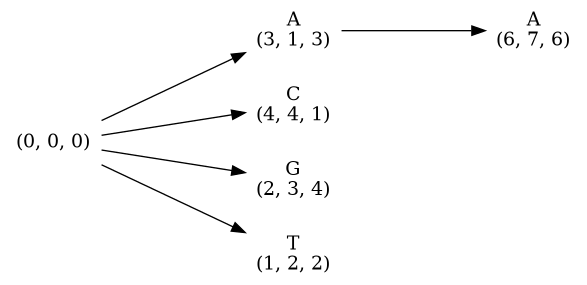
\includegraphics[width=0.5\textwidth]{Graph_4.png}
\end{wrapfigure}

Закончив перебирать алфавит для текущей вершины A (3, 1, 3) мы получим все вершины с которыми она имеет исходящую связь, т.е. вершины A (6, 7, 6), C (4, 4, 7), G (5, 3, 4) и T (7, 2, 5).
\clearpage
Таким образом, перебрав алфавит для всех вершин текущего слоя, мы получим все вершины следующего и их связи с текущим. NCSG на данном этапе построения приведен в \hyperref[ncsg:2]{приложении 6}, синим цветом отмечены связи не выходящие за пределы своего слоя.

\begin{wrapfigure}{r}{0.5\textwidth}
  \captionsetup{justification=centering}
  \caption*{\textbf{Приложение 6:} построение NCSG, 2 этап}
  \phantomsection
  \addcontentsline{toc}{subsubsection}{\textbf{Приложение 6:} построение NCSG, 2 этап}
  \label{ncsg:2}
  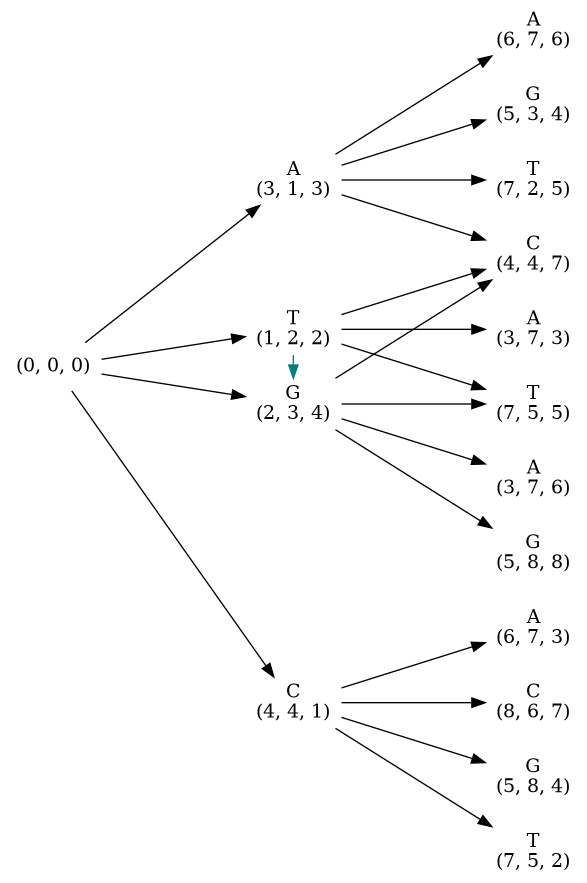
\includegraphics[width=0.5\textwidth]{Graph_5.png}
\end{wrapfigure}

Таким же образом необходимо получить все вершины следующего слоя, перебрав вершины полученного и так далее до тех пор, пока не закончится информация в таблицах. Если искомой координаты по текущему ключу и индексу в таблицах нет, значит мы пришли к конечной точке нашего NCSG, точке $(\infty, \infty, \infty)$.

Итоговый NCSG для последовательностей $S_{1} =$ TGACGATC, $S_{2} =$ ATGCTCAG и $S_{3} =$ CTAGTACG приведен в \hyperref[ncsg:3]{приложении 7}. Помимо межслоевых связей, есть так же связи не выходящие за пределы своего слоя, они помечены синим цветом. Следующим шагом необходимо избавиться от таких связей произведя прямую топологическую сортировку.

\subsection{Сортировка NCSG}

Для нахождения самого длинного пути из начала NCSG, в конец, который и будет являться наибольшей общей подпоследовательностью, необходимо произвести его прямую топологическую сортировку. Для этого напишем функцию \textit{ForwardTopSort}:

\begin{minted}[fontsize=\footnotesize, frame=lines, breaklines, breakafter=d, fontsize=\footnotesize, linenos]{python}

def ForwardTopSort(self, data): #На вход функции передаются список отсортированных последовательностей
    level_keys = set() #Ключи текущего слоя
    level_keys.add(self.sourcePoint) #Добавляем нулевую точку в качестве первого слоя
    layers = [] #Объявляем список множеств вершин каждого из слоев
    while len(level_keys) > 0:
        layers.append(level_keys) #Записываем готовый слой в переменную
        tmp_keys = set() #Временная переменная с множеством вершин текущего слоя
        for key in level_keys: #Перебераем вершины текущего слоя
            mustRemoved = set() #Множество ключей, с которыми нужно оборвать связи
            for link in self.ncsg[key]['out']: #Перебераем выходы текущей вершины
                if len(self.ncsg[link]['in'].difference(level_keys)) > 0: #Проверяем, есть ли у вершины связи с вершинами своего слоя
                    self.ncsg[link]['in'].discard(key) #Если такие связи есть, обрываем вход в текущую вершину для вершины предыдущего слоя
                    mustRemoved.add(link) #Записываем в переменную вершину, выход к которой необходимо оборвать
                else:
                    tmp_keys.add(link) #Если таких связей нет, записываем текущую вершину без изменений
            self.ncsg[key]['out'].difference_update(mustRemoved) #Обрываем выход из текущей вершины к записанной ранее
        level_keys = tmp_keys #Записываем готовые вершины текущего слоя
    return(layers)

\end{minted}

\begin{figure}[h!]
  \centering
  \caption*{\textbf{Приложение 7:} построенный \textit{Non-redundant Common Subsequence Graph} (NCSG)}
  \phantomsection
  \addcontentsline{toc}{subsubsection}{\textbf{Приложение 7:} построенный \textit{Non-redundant Common Subsequence Graph} (NCSG)}
  \label{ncsg:3}
  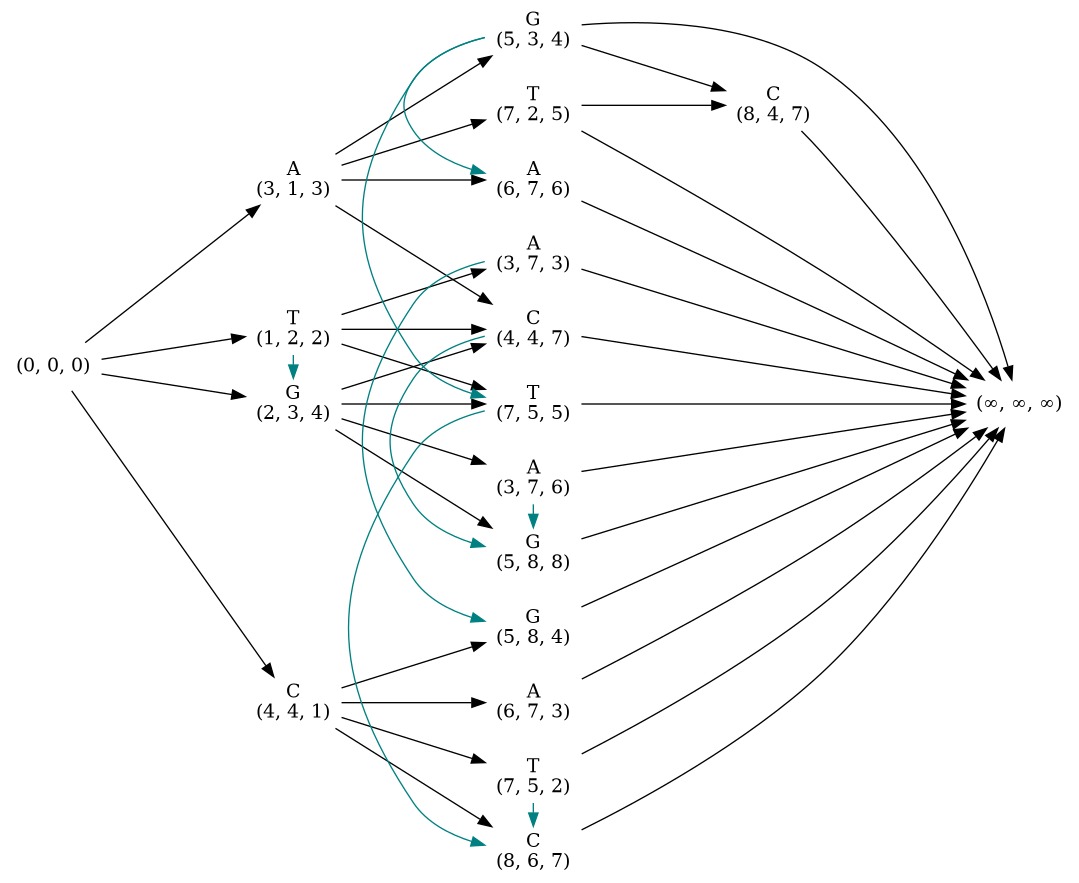
\includegraphics[width=0.9\textwidth]{Graph_1.png}
\end{figure}

Принцип действия данной сортировки заключается в следующем. Мы перебираем вершины по очереди каждого из слоев и если у вершины есть связь с вершиной своего же слоя, мы обрываем связь с вершиной предыдущего.

Рассмотрим на примере нашего NCSG, для последовательностей $S_{1}$, $S_{2}$ и $S_{3}$. Перебор слоев начинаем с первого, ему принадлежит только одна вершина $(0, 0, 0)$, а значит у данной вершины не может быть связей с другими вершинами своего слоя в силу отсутствия таких вершин. Теперь рассмотрим второй слой, его вершина G $(2, 3, 4)$ имеет входящую связь от вершины T $(1, 2, 2)$, в таком случае мы обрываем все связи данной вершины G $(2, 3, 4)$ с предыдущим слоем, тем самым перенося её на слой вперед.

\begin{wrapfigure}{l}{0.5\textwidth}
  \captionsetup{justification=centering}
  \caption*{\textbf{Приложение 8:} сортировка NCSG прямой топологической сортировкой}
  \phantomsection
  \addcontentsline{toc}{subsubsection}{\textbf{Приложение 8:} сортировка NCSG прямой топологической сортировкой}
  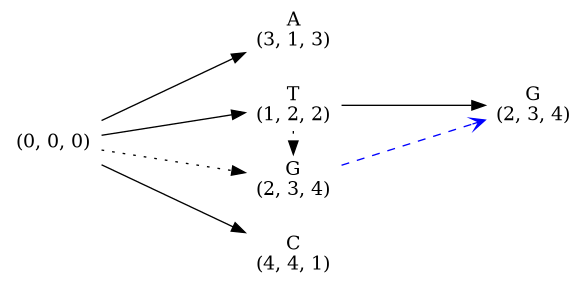
\includegraphics[width=0.445\textwidth]{Graph_6.png}
\end{wrapfigure}

Далее рассмотрим третий слой, он содержит 5 вершин имеющих входящие связи от других вершин этого слоя. Для каждой из них так же обрываем связи с предыдущим слоем. Таким образом, перебрав все слои мы получим граф показанный ниже. Если после рассматриваемого слоя есть ещё один слой с которым данная вершина не имеет связи, путь к данной вершине мы в дальнейшем не рассматриваем, т.к. такой путь не является самым длинным. Не рассматриваемые пути обозначены красным цветом.
\begin{figure}[h!]
  \centering
  \caption*{\textbf{Приложение 9:} NCSG отсортированный прямой топологической сортировкой}
  \phantomsection
  \addcontentsline{toc}{subsubsection}{\textbf{Приложение 9:} NCSG отсортированный прямой топологической сортировкой}
  \label{ncsg:4}
  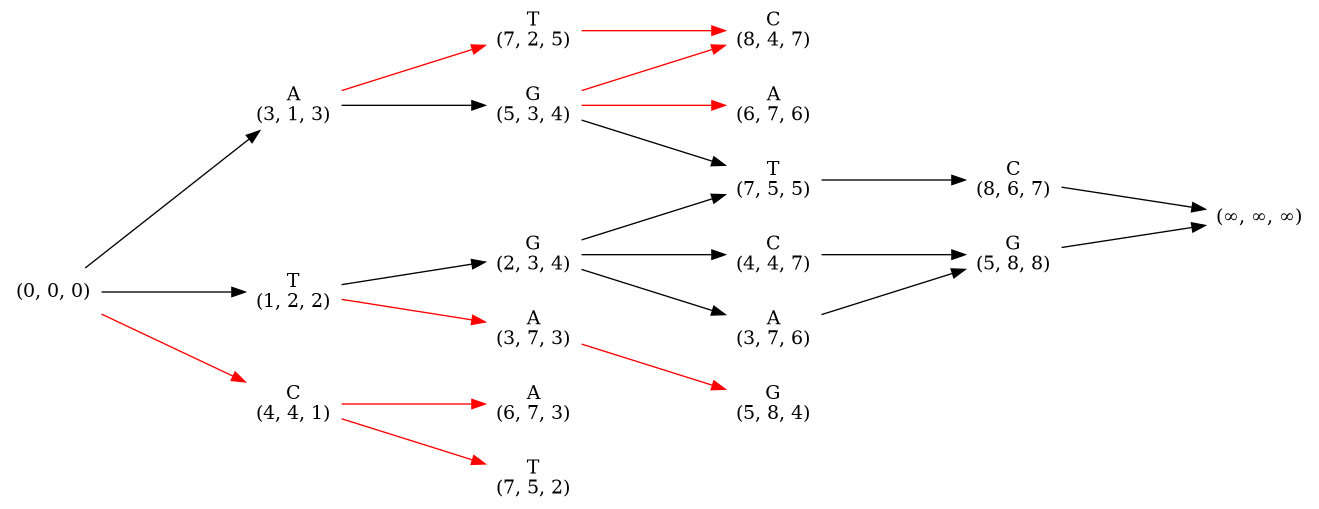
\includegraphics[width=1\textwidth]{Graph_2.png}
\end{figure}

\subsection{Чтение NCSG}

Самые длинные пути отсортированного NCSG и являются искомыми MLCS. Однако отсортированный NCSG содержит как самые длинные, так и менее длинные пути, отмеченные красным цветом в \hyperref[ncsg:4]{приложении 9}. Во избежание таких, неподходящих путей, прочитаем полученный NCSG задом наперед. Для этого напишем следующую функцию:

\begin{minted}[fontsize=\footnotesize, frame=lines, breaklines, breakafter=d, fontsize=\footnotesize, linenos]{python}

def GetMLCS_3(self):
    def dfs_paths(graph, start, goal):
        paths = [] #Переменная, в которую мы будем записывать найденные пути
        stack = [(start, [start])] #Переменная, в которую мы временно записываем вершины и пути к ним
        while stack:
            (vertex, path) = stack.pop() #Рассматриваем последнюю вершину из переменной stack и путь к ней
            for next in graph[vertex]['in']: #Перебираем все вершины входящие в данную
                if next == goal: #Проверяем, является ли вершина входящая в данную начальной точкой (0, 0, 0)
                    paths.append(path[1:]) #Если да, записываем полученный путь в переменную paths
                else:
                    stack.append((next, path + [next])) #В противном случае записываем входящую вершину и путь к ней в переменную stack
        return paths #Функция возвращает список всех путей из конца NCSG в начало
    paths = dfs_paths(self.ncsg, self.sinkPoint, self.sourcePoint) #Получаем список всех путей из конца NCSG в начало
    sequences = []
    for path in paths: #Перебираем полученные пути
        sequence = []
        for key in reversed(path): #Перебираем вершины текущего пути из начала в конец
             sequence.append(self.ncsg[key]['char']) #Формируем подпоследовательности начальных последовательностей
        sequences.append(sequence) #Записываем найденную подпоследовательность
    return(sequences)

\end{minted}

\begin{wrapfigure}{l}{0.3\textwidth}
  \captionsetup{justification=centering}
  \caption*{\textbf{Приложение 10:} чтение NCSG, 1 этап}
  \phantomsection
  \addcontentsline{toc}{subsubsection}{\textbf{Приложение 10:} чтение NCSG, 1 этап}
  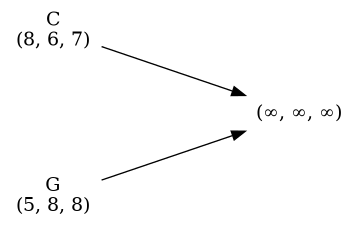
\includegraphics[width=0.3\textwidth]{Graph_7.png}
\end{wrapfigure}

Чтение NCSG происходит следующим образом. В качестве начальной точки для чтения выбираем конечную точку NCSG, точку $(\infty, \infty, \infty)$. Для данной вершины перебираем все в неё входящие и проверяем, нет ли среди этих, входящих вершин, начальной точки NCSG, точки $(0, 0, 0)$. Если нет, запоминаем каждую входящую вершину и пути к ним. Теперь, после того как мы перебрали все входящие в данную вершину точки, рссмариваем каждую из полученных вершин.
\begin{figure}[h!]
  \caption*{\textbf{Приложение 11:} чтение NCSG, 2 этап}
  \phantomsection
  \addcontentsline{toc}{subsubsection}{\textbf{Приложение 11:} чтение NCSG, 2 этап}
  \label{ncsg:5}
  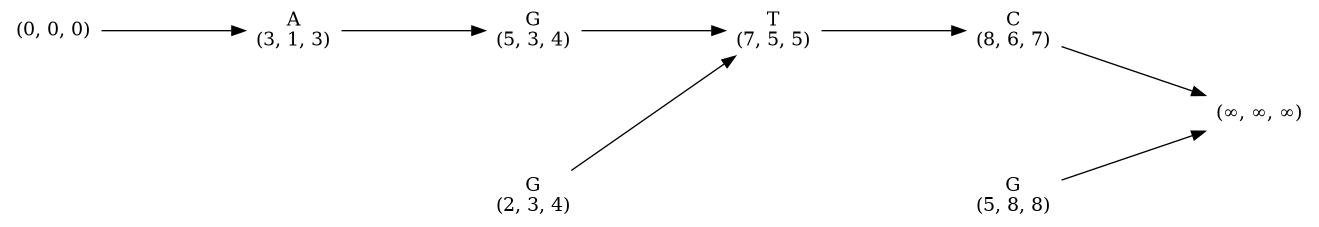
\includegraphics[width=1\textwidth]{Graph_8.png}
\end{figure}

Для каждой из них снова перебираем все входящие и так далее до тех пор, пока среди входящих вершин текущей не окажется начальная точка NCSG, точка $(0, 0, 0)$, это будет означать что мы прочитали весь путь и получили все его элементы. Далее возвращаемся к одной из вершин без входящих связей, на примере в \hyperref[ncsg:5]{приложении 11} это вершины G $(2, 3, 4)$ и G $(5, 8, 8)$, и проделываем для неё то же самое, находя все элементы ещё одного пути.
\begin{figure}[h!]
  \caption*{\textbf{Приложение 12:} чтение NCSG, 3 этап}
  \phantomsection
  \addcontentsline{toc}{subsubsection}{\textbf{Приложение 12:} чтение NCSG, 3 этап}
  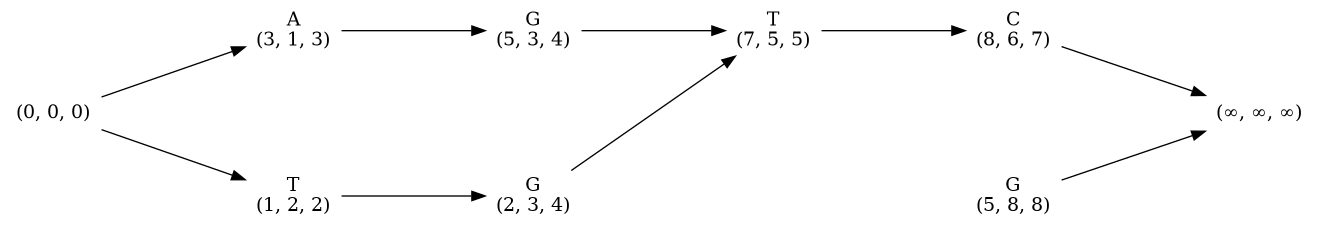
\includegraphics[width=1\textwidth]{Graph_9.png}
\end{figure}

Проделывая данную операцию мы получаем все наибольшие пути NCSG, в конечном счете мы получим граф содержащий пути одинаковой длины, такой граф для последовательностей $S_{1}$, $S_{2}$ и $S_{3}$ приведен в \hyperref[ncsg:6]{приложении 13}.
\begin{figure}[h!]
  \caption*{\textbf{Приложение 13:} чтение NCSG, 4 этап}
  \phantomsection
  \addcontentsline{toc}{subsubsection}{\textbf{Приложение 13:} чтение NCSG, 4 этап}
  \label{ncsg:6}
  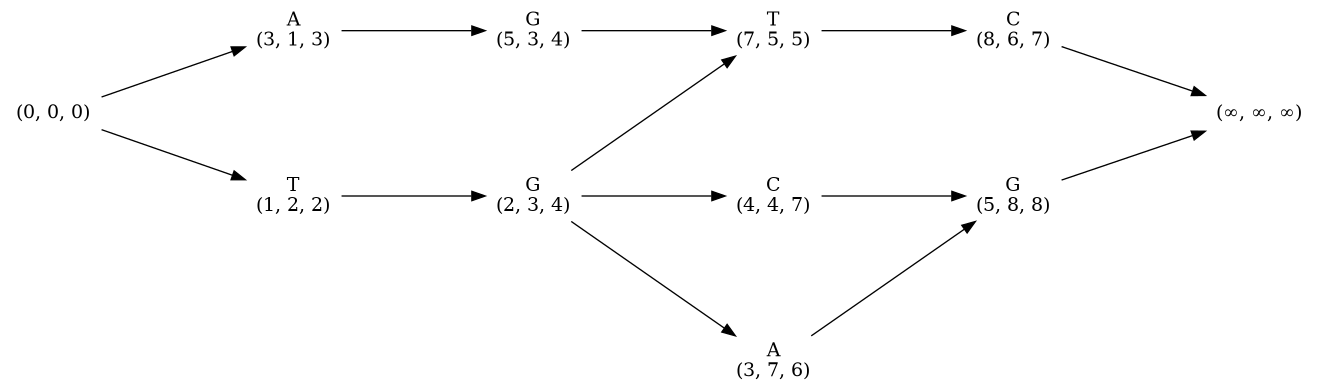
\includegraphics[width=1\textwidth]{Graph_3.png}
\end{figure}

Теперь достаточно выписать элементы каждого из путей в направлении отсортированного NCSG, т.е. из начальной точки $(0, 0, 0)$ к конечной $(\infty, \infty, \infty)$. В нашем случае возможно четыре различных пути, а значит мы получили четыре MLCS для последовательностей $S_{1}$, $S_{2}$ и $S_{3}$:
\[S_{1} = TFGACGADTC \quad S_{2} = ATGLCTCAFG \quad S_{3} = CTADGTALCG\]
\begin{multicols}{2}
  \begin{itemize}[leftmargin=-0cm]
          \centering
    \item $MLCS_{1}$ = AGTC \item $MLCS_{2}$ = TGTC
    \item $MLCS_{3}$ = TGCG \item $MLCS_{4}$ = TGAG
  \end{itemize}
\end{multicols}

\section{Исследования с использованием алгоритма MLCS}

Практически важен для применения в биоинформатике алфавит длиной 4 символа $\Sigma_{4} = \left\{A, C, G, T\right\}$ как часть природных ДНК последовательностей. С помощью реализованного алгоритма исследуем некоторые интересные зависимости полученных LCS. Для этого сгенерируем 1000 случайных наборов из трех последовательностей длиной по 50 символов и алфавитом 4 символа каждая. Сразу обратило на себя внимание количество полученных LCS. Их количество доходило до 2107. В \hyperref[diog:1]{приложении 14} приведена гистограмма вероятностей полученного количества LCS. В 95\% случаях количество LCS было меньше 260.

\begin{figure}[h!]
  \caption*{\textbf{Приложение 14: }Гистограмма вероятностей количества LCS}
  \phantomsection
  \addcontentsline{toc}{subsubsection}{\textbf{Приложение 14: }Гистограмма вероятностей количества LCS}
  \label{diog:1}
  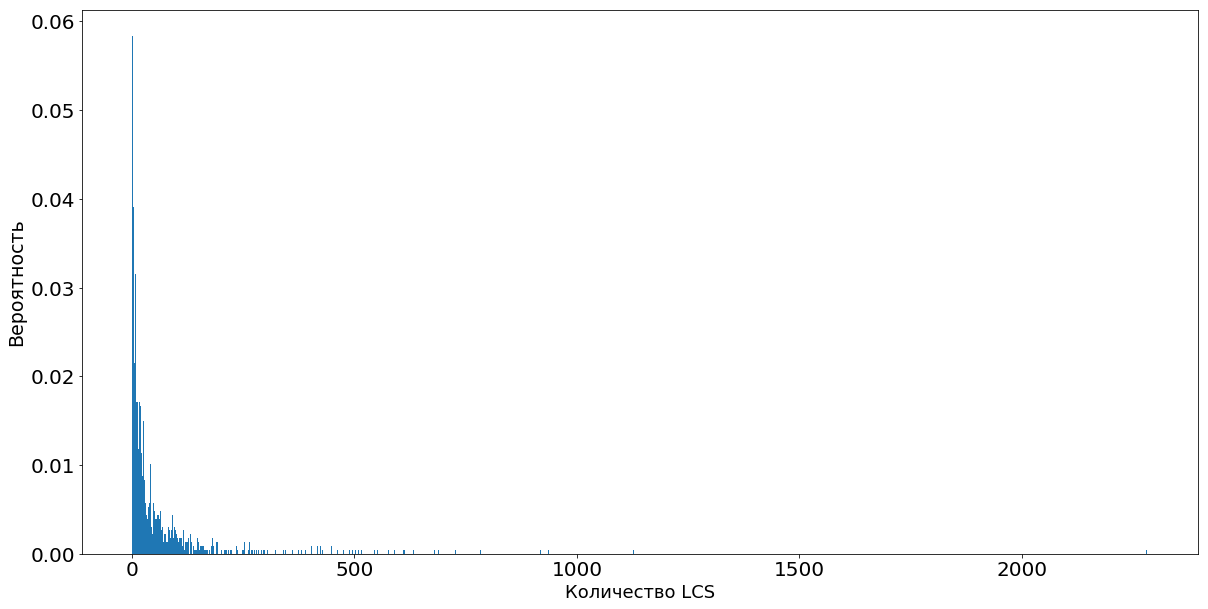
\includegraphics[width=1\textwidth]{Diogram_1.png}
\end{figure}

\begin{figure}[h]
  \centering
  \begin{subfigure}{.5\textwidth}
    \centering
    \captionsetup{justification=centering}
    \caption*{\textbf{Приложение 15:} Соотношение между длинами получаемых LCS и их количеством}
    \phantomsection
    \addcontentsline{toc}{subsubsection}{\textbf{Приложение 15: }Соотношение между длинами получаемых LCS и их количеством}
    \label{diog:2}
    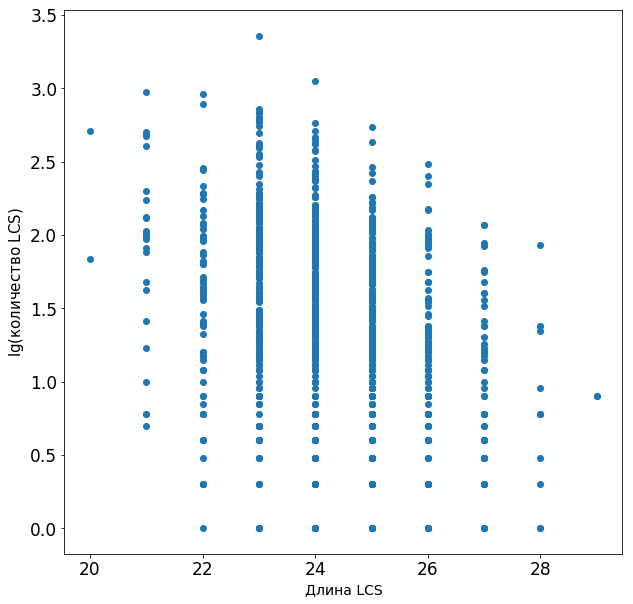
\includegraphics[width=0.9\textwidth]{Diogram_2.png}
  \end{subfigure}%
  \begin{subfigure}{.5\textwidth}
    \centering
    \captionsetup{justification=centering}
    \caption*{\textbf{Приложение 16:} Гистограмма распределения вероятностей длин LCS}
    \phantomsection
    \addcontentsline{toc}{subsubsection}{\textbf{Приложение 16: }Гистограмма распределения вероятностей длин LCS}
    \label{diog:3}
    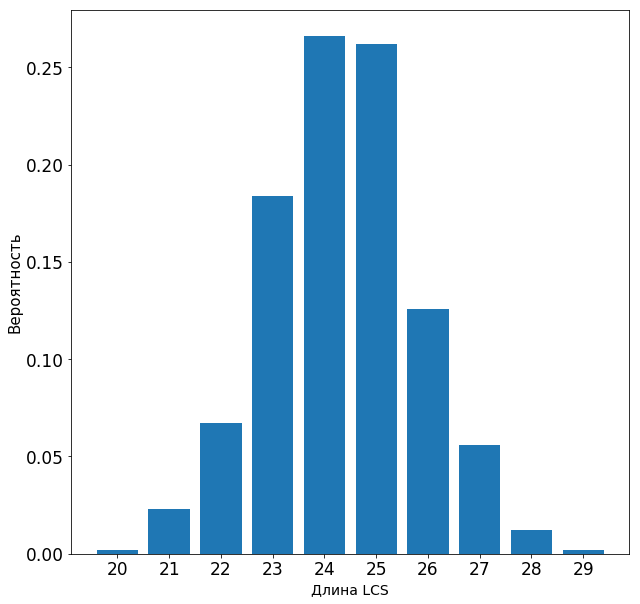
\includegraphics[width=0.9\textwidth]{Diogram_3.png}
    \label{fig:sub2}
  \end{subfigure}
  \vspace{-0.5cm}
\end{figure}
В \hyperref[diog:2]{приложении 15} приведено соотношение между длинами получаемых LCS и их количеством для наборов из трех последовательностей длиной 50 элементов и алфавитом 4. Количество LCS приводится в логарифмическом масштабе. Длины полученных LCS лежат в довольно узком диапазоне их распределение вероятностей схоже с нормальным распределением со средним $\bar{n} = 24.345$ и среднеквадратичным отклонением $\sigma = 1.44$. В \hyperref[diog:3]{приложении 16} приводится гистограмма распределения вероятностей длин LCS.

\section{Итоги исследования}

За время выполнения работы мы реализовали алгоритм Linear-MLCS на языках программирования Python и C++, в том числе метод построения NCSG графа, его чтения, а так же методы прямой и обратной топологических сортировок. Описали работу алгоритма на примере его реализации на языке Python. Провели исследования зависимостей количества полученных LCS от их длины, определили распределение вероятностей длин LCS и их количества.

Коды реализаций алгоритма на языках Python и C++ доступны на GitHub по ссылке \href{https://github.com/Garison1/MLCS-research}{https://github.com/Garison1/MLCS-research}.
\nocite{*}



\end{document}

% Local Variables:
% LaTeX-command: "latex -shell-escape"
% End:
